\documentclass[../main.tex]{subfiles}
\graphicspath{{\subfix{../../images/}}}
\begin{document}

\chapter{More Results}\label{chap:more_results}

\bigskip
\begin{quote}
  \emph{My view is that language and the hand have a certain common agenda--- that is, they enable us to \textbf{grasp} things: to pin them down and make them useful. And we cannot deny that they have done that in spades. They have helped us to use the world and, by doing so, to develop many of the things of which we are most justly proud, the fruits of civilization.}
  
  \raggedleft{--- Iain McGilchrist, \emph{Ways of Attending, 2016}}
\end{quote}

\cleardoublepage%

% Data Manifold 
  % Trajectories show this X pattern 
  % Develop a toy GMM models
  % discuss log transforming
  % Does subspace confinement correlate with performance? Does subspace confinement change over trials?

% PCA stuff
% explain how this might be missing the point, because our data isn't gaussian!
% but we can show how our data accords with the literature, but we can be more careful in our analysis

% Mixture Modeling
  % GMMs as an attempt to overcome the spikiness of the data manifold
  % Do GMMs live mostly on or off manifold? I.e. what happens with the off-manifold activity over learning? Increase, decrease, or stay the same?
  % Does variance increase / decrease / non-monotonic?
  % Do models become more self-similar? (derivative/ difference)
  % Do models become more or less similar to prior?

% Intro to Null space -- Optimization solutions
  % Are subject solutions attending to the nullspace? or are they more aligned to their "natural repertoire"

% Null Space Analysis – PCA on the nullspace, information from the nullspace activity

% Do GMMs over learning become more self-similar? Does the variance/entropy/complexity decrease?

% Are GMM fits influenced by the prior?

% Does an optimization-based solution approach support model-free learning?

% Do subjects attend to the null space?

% What does it mean to have high / low null space activity?
% 	Show stats, discuss why / why not
% 	Does this change across learning?
% What does activity look like in the "null" (task-irrelevant) vs. "non-null" (task-relevant) space? The literature hypothesizes that subjects should attend to variability in the task-relevant subspace of their muscle activity. 
% Hypothesis: in line with prior studies, that we will see lower variability in the task-relevant subspace compared with the task-irrelevant subspace in later trials.
% Hypothesis: over trials, task-relevant variability will decrease as subjects identify the task-relevant dimensions of their movement space.


\section{Structure of the Data Manifold}


\subsection{Is EMG Lognormal?}

Brief intro into log-normality of the data

Also show correlations between channels and introduce the idea of subspace confinement

Motivate the shape of the manifold discussion next

\begin{figure}[H]
    \centering
    \includegraphics[width=1.0\textwidth]{more_results/pairplot/raw_pairplot.png}
    \caption[Pairplot of calibration data]{Pairplot of calibration data}\label{fig:raw_pairplot}
\end{figure}

\begin{figure}[H]
    \centering
    \includegraphics[width=1.0\textwidth]{more_results/pairplot/log_pairplot.png}
    \caption[Pairplot of log-transformed calibration data]{Pairplot of log-transformed calibration data}\label{fig:log_pairplot}
\end{figure}




Structure of data manifold → multimodal, spiky, etc. means we have to be careful about statistics
	Motivate PCA vs mixture models
	Show PCA and mixture model fits
Do we see shifts over learning under different models?
	Fit models across learning, use the stats to show shifts?
Entropy of GMM model fits over trials? “Policy entropy”? (Bits of information contained in the policy? [0,1] % → [inf,0] bits – the more high-probability actions, or concentration around a few actions, the less entropy, the lower the description length. Balance between exploration and exploitation.
Does a subject penalize changes to their controllers/action distribution? Do they follow a KL-divergence type of measurement when improving their policy? Do we see this in the dynamics of the statistics over trials?

``SUBSPACE CONFINEMENT''

The fits enable you to overcome the subspace confinement, give us a reasonably tractable model of our multimodal data. Weve proven that the data lies in distinct, low-dimensional subspaces of the activity space. The GMMs describe this fact, particularly the rank of the variances.	
Explain what these fits are, visualize comparisons to data, prove that theyre reasonable
Motivate the GMM fitting with the overview of the data as a model to capture stats
!!! you cant recover the subspace-confinement if you look at the combined covariance (if subspaces overlap) – this means analyzing bulk covariances will hide subspace confinement in the data. This could be happening even at the intra-trial level
Explain how the data is very sparse! Each trajectory is very low-probability. The trajectories are very thin, subjects repeat movements which are common, this is whats captured by the GMM


How many discrete movements make up a trajectory? How do we define a discrete movement? Can we define a segmentation for movements, and use this as a measure of “smoothness” of control?
Hypothesis: movement modularity or segmentation decreases over learning as subjects discover smoother solutions to the task. These movement segments are part of the subjects natural movement repertoire.
Do subjects freeze degrees of freedom to simplify the learning task? (E.g. How many PCA components are active at once, how does this change over time?)
Hypothesis: early in learning subjects will activate only a subset of available movement dimensions as defined by task-space movement repertoire, PCA or similar model of variability.
If we compute PCA on each trial, does the dimensionality increase, decrease, or something else over trials? The answer points to exploration vs. exploitation, hierarchical or mixed-controller solutions. This may highlight how the structure of variability develops over trials. 
Hypothesis: Early in learning, subjects will explore more, and their dimensionality will be high (similar to the dimensionality of natural movement or the calibration task). Over learning, dimensionality will decrease as subjects “hone in” on solutions to the task. 
Dig into subjects movement policies– what structure is there? Are subjects choosing from a repertoire of policies (e.g. learning one policy for each target, a kind of hierarchical policy, or learning the decoder directly to flexibly produce movement solutions?)
Hypothesis: subjects are doing everything all at once– theyre internalizing the decoder by learning an internal model (a mapping from targets to movements) of their new environment, and theyre using targets as cues to remember discrete movements. This is highlighted when subjects make incorrect movements– how they recover from these mistakes will highlight the difference between an internal model and model-free learning.
Hypothesis: Early in learning, well see subjects repeat many of the same movements as theyre repeating what works in a model-free manner. Later in learning, well see subjects responding more flexibly, having developed a better internal model of the movement-task contingency. 
NB: these hypotheses contradict other hypotheses about exploration. If subjects are optimally exploring the space, collecting data about the contingency, they wouldnt be making the same movements repeatedly, they would be making a variety of movements. This might come down to individual subjects strategies for how they approach the task. We may see some subjects choosing to explore, rather than solve the task. Other subjects may be focused on solving the task and learning through their mistaken movements.
Can we take the first movement segment (of each block?) as representing subjects predictive forward models? Does this give us an indication of subjects' forward models? Or of their discrete policy decision memory? Do these get better over trials?
Hypothesis: Early in learning, these “first corrections” will be poor, in the sense that they will often be incorrect and likely default back to some common movement policy (perhaps a movement from the natural movement dataset?). Late in learning, well begin to see more flexible, assumedly internal-model driven responses to these “mistakes”. 
Are subjects using one controller or several? Are they composing them or switching between them? Are they learning which controller to switch between or are they developing a single controller to solve for all targets? Does this explain perturbation response? Subjects might be building p(best controller | target, state), that is choosing from distinct policies, rather than developing a de novo policy.
Hypothesis: Subjects are doing everything at once: they are internalizing a model of the task dynamics and decoder to form a general controller/policy, they are forming or recalling individual controllers/policies for individual targets. We can investigate this by looking within trial trajectories, where we should be able to classify behavior as policy switching/activation vs. generic controller/policy response.

Dig into the data, what does it look like from different angles?
Means in EMG and task space
Activity distributions in EMG and task space
Covariance structure?
Tangent space?
Manifold structure – UMAP over time? Colorful plot showing shift over time… 
Discuss trajectory, data scaling
On what scale (trials, timesteps) is the model altered? the policy? →
What does the trial-to-trial variance look like?
Subtract out the mean trajectory?

If nothing so far really explains subjects performance, including the decoder / task contingency itself, then the constraints imposed on subjects must come from the subjects themselves, from their data manifold.
Discuss the geometry of the task; weve shown that aspects of the decoder arent predictive of subjects success– so something else (the data manifold itself!) is responsible for performance.
Go deeper into the decoder– were inverting the mapping from latent “activations” to emg to get an emg-to-latent mapping which is norm-minimizing 
What is the structure of the data manifold? 
Show/explain the concept of subspace confinement
The data isnt Gaussian, so PCA is going to suffer
This is a really important point we can make – looking at the data manifold, PCA will give us something but its going to hide a lot of information about subspace confinement, covariance structure, etc. Its essentially going to align the axes towards high-variance directions, but not take into account the “spikey” nature of the data manifold. This will give us a false sense of the correlation structure between EMG channels.
In other studies, theyve analyzed surface EMG data with PCA to then say that since there are high-variance components that capture gross hand postures / movements, and lower-variance, higher-order components that capture finer movements, this implies something about the neural basis for hand control. While it may, this result via PCA isnt surprising. What is more insightful is to understand the underlying structure of the data manifold, and follow its changes across learning to understand how the motor system copes with a new environment. We can clearly show how PCA misses an important aspect of the data manifold, its highly nonlinear structure, and how this plays a role in subjects performance and learning.
We can highlight this by showing PCA projections of the data colored to show how theyre mixed in terms of their target, etc. – not getting good separation of the data because of the non-gaussian manifold



\section{How Does PCA Dimensionality Compare Across Tasks?}

Show dimensionality of different tasks

Show two-dimensional projections of activity

Look at these PCA modes, compare them to natural movement...? Are these modes relevant to the task? Hmm....

“Movement” session Compare this to calibration, trial in terms of e.g. entropy to show that subjects are moving beyond their  “Calibration” session

Hypothesis: subjects explore beyond their natural movements in the calibration task.


\begin{figure}[H]
  \centering
  \includegraphics[width=1.0\textwidth]{more_results/pca_dimensionality/PCA_variance.pdf}
  \caption[Explained variance over tasks]{No correlation!}\label[figure]{pca_variance}
\end{figure}


% \clearpage
% \begin{table}[H]
% \begin{center}
%     \caption{$p$-values for \Cref{pca_variance}}\label{table:pvalues}
%     \begin{tabular}{l | c}
%         Variable & $p$ Value \\
%         \hline
%         \cellcolor{red!25} Calibration --- Movement & \cellcolor{red!25} 9.644e-09 \\
%         \cellcolor{red!25} Trial Block 1 --- Movement & \cellcolor{red!25} 9.348e-05 \\
%         Trial Block 1 --- Calibration & 5.684e-01 \\
%         \cellcolor{red!25} Trial Block 2 --- Movement & \cellcolor{red!25} 5.591e-05 \\
%         Trial Block 2 --- Calibration & 6.444e-01 \\
%         Trial Block 2 --- Trial Block 1 & 1.000e+00 \\
%         \cellcolor{red!25} Trial Block 3 --- Movement & \cellcolor{red!25} 1.255e-02 \\
%         \cellcolor{red!25} Trial Block 3 --- Calibration & \cellcolor{red!25} 4.340e-02 \\
%         Trial Block 3 --- Trial Block 1 & 8.755e-01 \\
%         Trial Block 3 --- Trial Block 2 & 8.230e-01 \\
%         \cellcolor{red!25} Trial Block 4 --- Movement & \cellcolor{red!25} 2.040e-02 \\
%         \cellcolor{red!25} Trial Block 4 --- Calibration & \cellcolor{red!25} 2.786e-02 \\
%         Trial Block 4 --- Trial Block 1 & 8.039e-01 \\
%         Trial Block 4 --- Trial Block 2 & 7.394e-01 \\
%         Trial Block 4 --- Trial Block 3 & 1.000e+00 \\
%         \cellcolor{red!25} Trial Block 5 --- Movement & \cellcolor{red!25} 2.762e-02 \\
%         \cellcolor{red!25} Trial Block 5 --- Calibration & \cellcolor{red!25} 2.058e-02 \\
%         Trial Block 5 --- Trial Block 1 & 7.487e-01 \\
%         Trial Block 5 --- Trial Block 2 & 6.783e-01 \\
%         Trial Block 5 --- Trial Block 3 & 1.000e+00 \\
%         Trial Block 5 --- Trial Block 4 & 1.000e+00 \\
%         \end{tabular}
% \end{center}
% \end{table}


\begin{figure}[H]
  \centering
  \includegraphics[width=1.0\textwidth]{more_results/pca_dimensionality/pca_pvalues.pdf}
  \caption[Explained variance Tukey test]{$p$-values for Tukey's honestly significant difference test for pairwise means of a group of samples. Here we compare the explained variance of the top two singular values for the movement, calibration, and 5 blocks of task trials over subjects.}\label{fig:pca_pvalues}
\end{figure}

\Cref{fig:pca_pvalues}

% The observations being tested are independent within and among the groups.
% The groups associated with each mean in the test are normally distributed.
% There is equal within-group variance across the groups associated with each mean in the test (homogeneity of variance).



% \begin{figure}[H]
% \phantomsection\label{fig:PCA_trial_variance}
% \centering
% 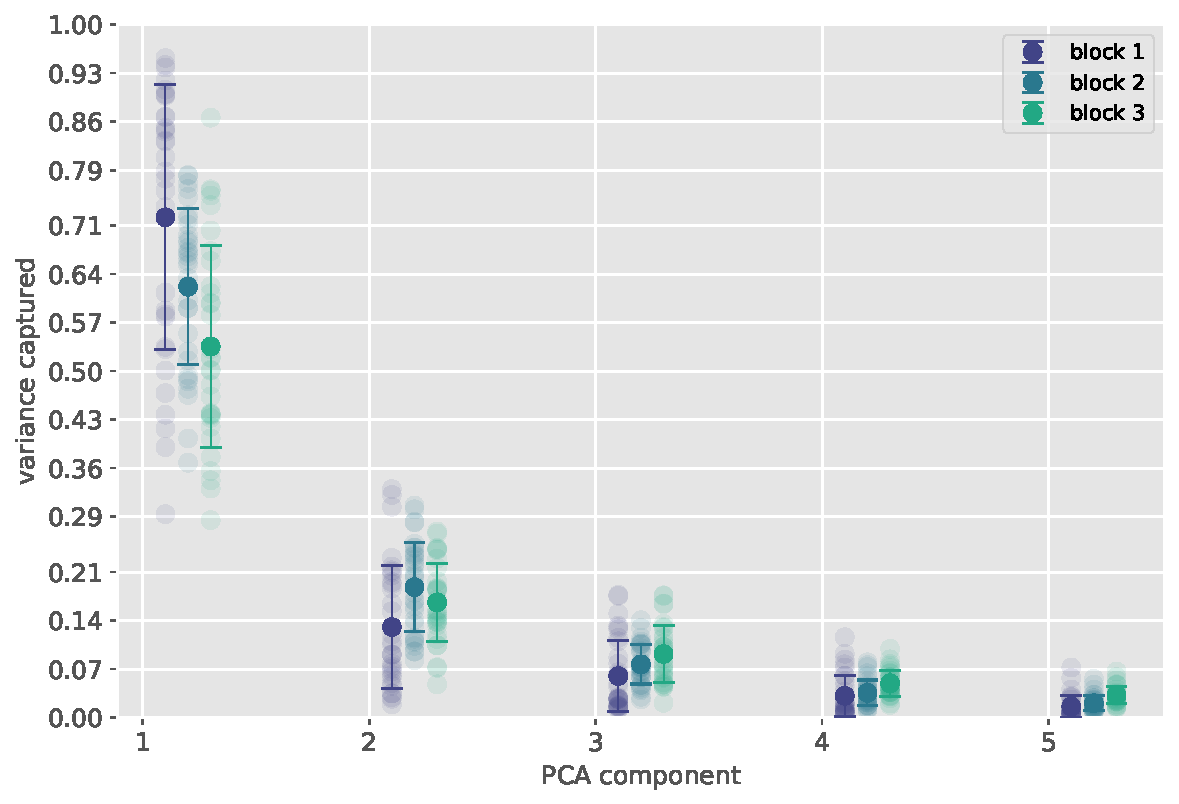
\includegraphics[width=0.2\textwidth]{images/data_analysis/center_hold/PCA_trial_variance.pdf}
% \caption{Fraction of variance captured by the top five principle components when PCA is run on the EMG time series' of individual trials of the center-hold, reach-out task. Error bars are standard deviation. Over blocks, we see a slight decrease in the mean of the top component's variance fraction, though with high variance. This may suggest greater exploration within-trial, as less variance is captured by a single component over blocks, though it could reflect more varied dynamics across trials as the subject discovers new, task-relevant activations.}\label{fig:PCA_trial_variance}
% \end{figure}

% We might model this task as the subject selecting an EMG signal $x$ which minimizes the distance between a target position $b$ and the projection of the EMG signal through the mapping $M$ as well as minimizes the norm of $x$ in order to conserve metabolic energy. This optimization can be written as a regularized least squares problem:

% \begin{align}
%   \min_x\frac{1}{2}||Mx - b||^2_2 + \frac{\lambda}{2}||x||_2^2.
% \end{align}

% This problem is known to have a unique minimum for $\lambda>0$ which is an approximation $Mx\approx b$ regardless of the shape or rank of $M$. This implies that the subject, if they are biophysically capable to do so, will learn distinct motor outputs for each target rather than reusing modes for multiple targets with different activation levels. That is the subject will, over time, learn to fractionate their muscle output to reach their goal in order to minimize effort. For instance, to reach the the target at position $(1,0)$ in Cartesian coordinates, the subject could activate a bespoke activity mode and activate a combination of two or more modes for targets at $\pm45^\circ$ from this central target. If this is the case, the model predicts that the dimensionality of the EMG signal will increase over the course of training as the subject learns to construct bespoke activity modes for each target.


% In \Cref{fig:PCA_concat_variance} we compute PCA on the concatenation of all trials within blocks for which we predict an increase in the number of dominant EMG modes as subjects learn multiple movements to reach individual targets. We expect subjects to, over time, develop some number of bespoke movement modes to activate independently and as a composition to reach each target. We find a suggestion of this idea in the data with our basic PCA analysis. More trials, session, and subjects will be required to explore this idea, and we are investigating probabilistic measures of signal complexity such as entropy to formalize this hypothesis. One direction might be to further define this task a regularized regression with different regularization terms chosen normatively for different sections of the learning and control process, and fitting data to these predictions. For instance, early in training subjects may not optimize for target accuracy as much as for signal sparsity, whereas later in learning subjects may optimize for target accuracy and output signal magnitude.

% \begin{figure}[H]
% \phantomsection\label{fig:PCA_concat_variance}
% \centering
% 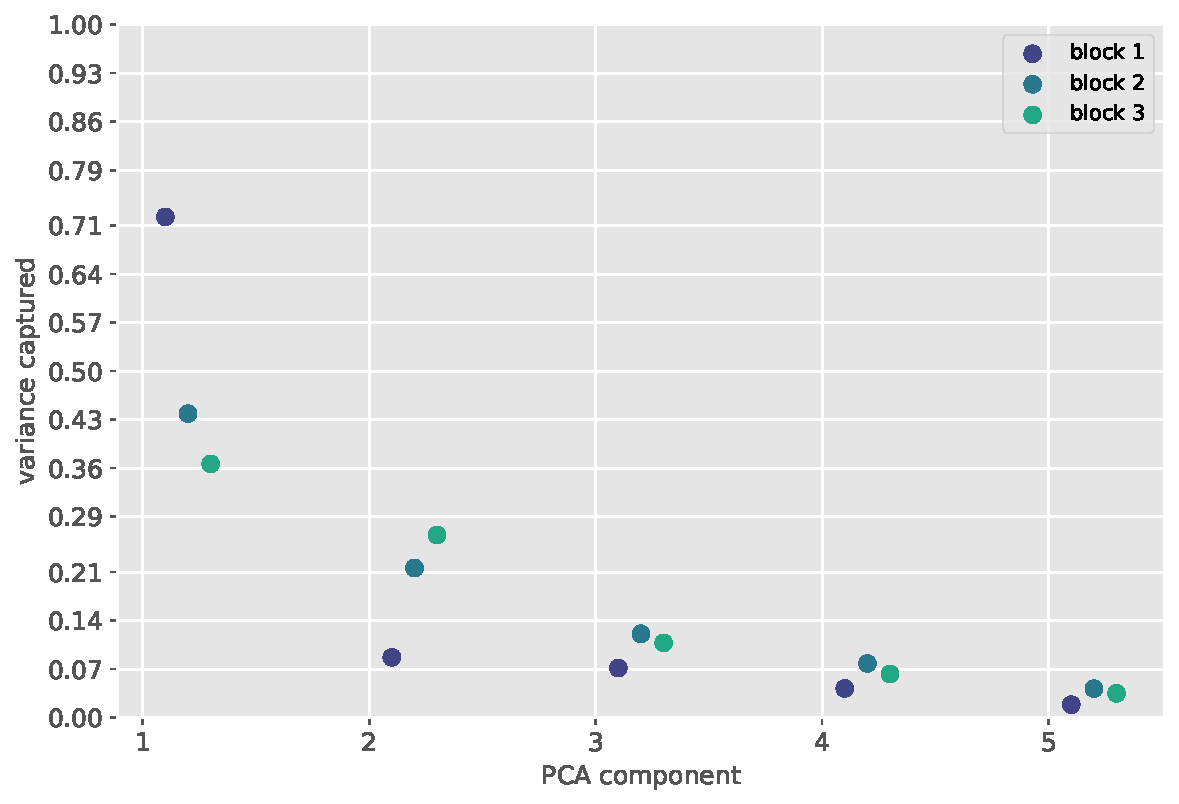
\includegraphics[width=0.2\textwidth]{images/data_analysis/center_hold/PCA_concat_variance.pdf}
% \caption{Fraction of variance captured by PCA computed on concatenated EMG time series concatenated over trials. Over blocks, we see variance shifting from the top component to other components. We hypothesize that across learning we would see the development of bespoke modes used in combination to reach individual targets. This would predict an increase in the complexity of the EMG time series over learning. Here we see suggestions of this prediction.}\label{fig:PCA_concat_variance}
% \end{figure}


% We first asked whether PCA applied to each individual trial would extract a single, high-variance component reflecting the dimensionality of the behavior. Since each finger movement is intuitively one dimensional, we predict that PCA would find a single high-variance component when run on each individual trial. As shown in \Cref{fig:PCA_variances}, this is generally the case, though there are some outlier trials. After inspecting these outlier trials, it is likely that the subject moved multiple fingers in these trials counter to the experimenter's instruction.

% \begin{figure}[H]
% \phantomsection\label{fig:PCA_variances}
% \centering
% 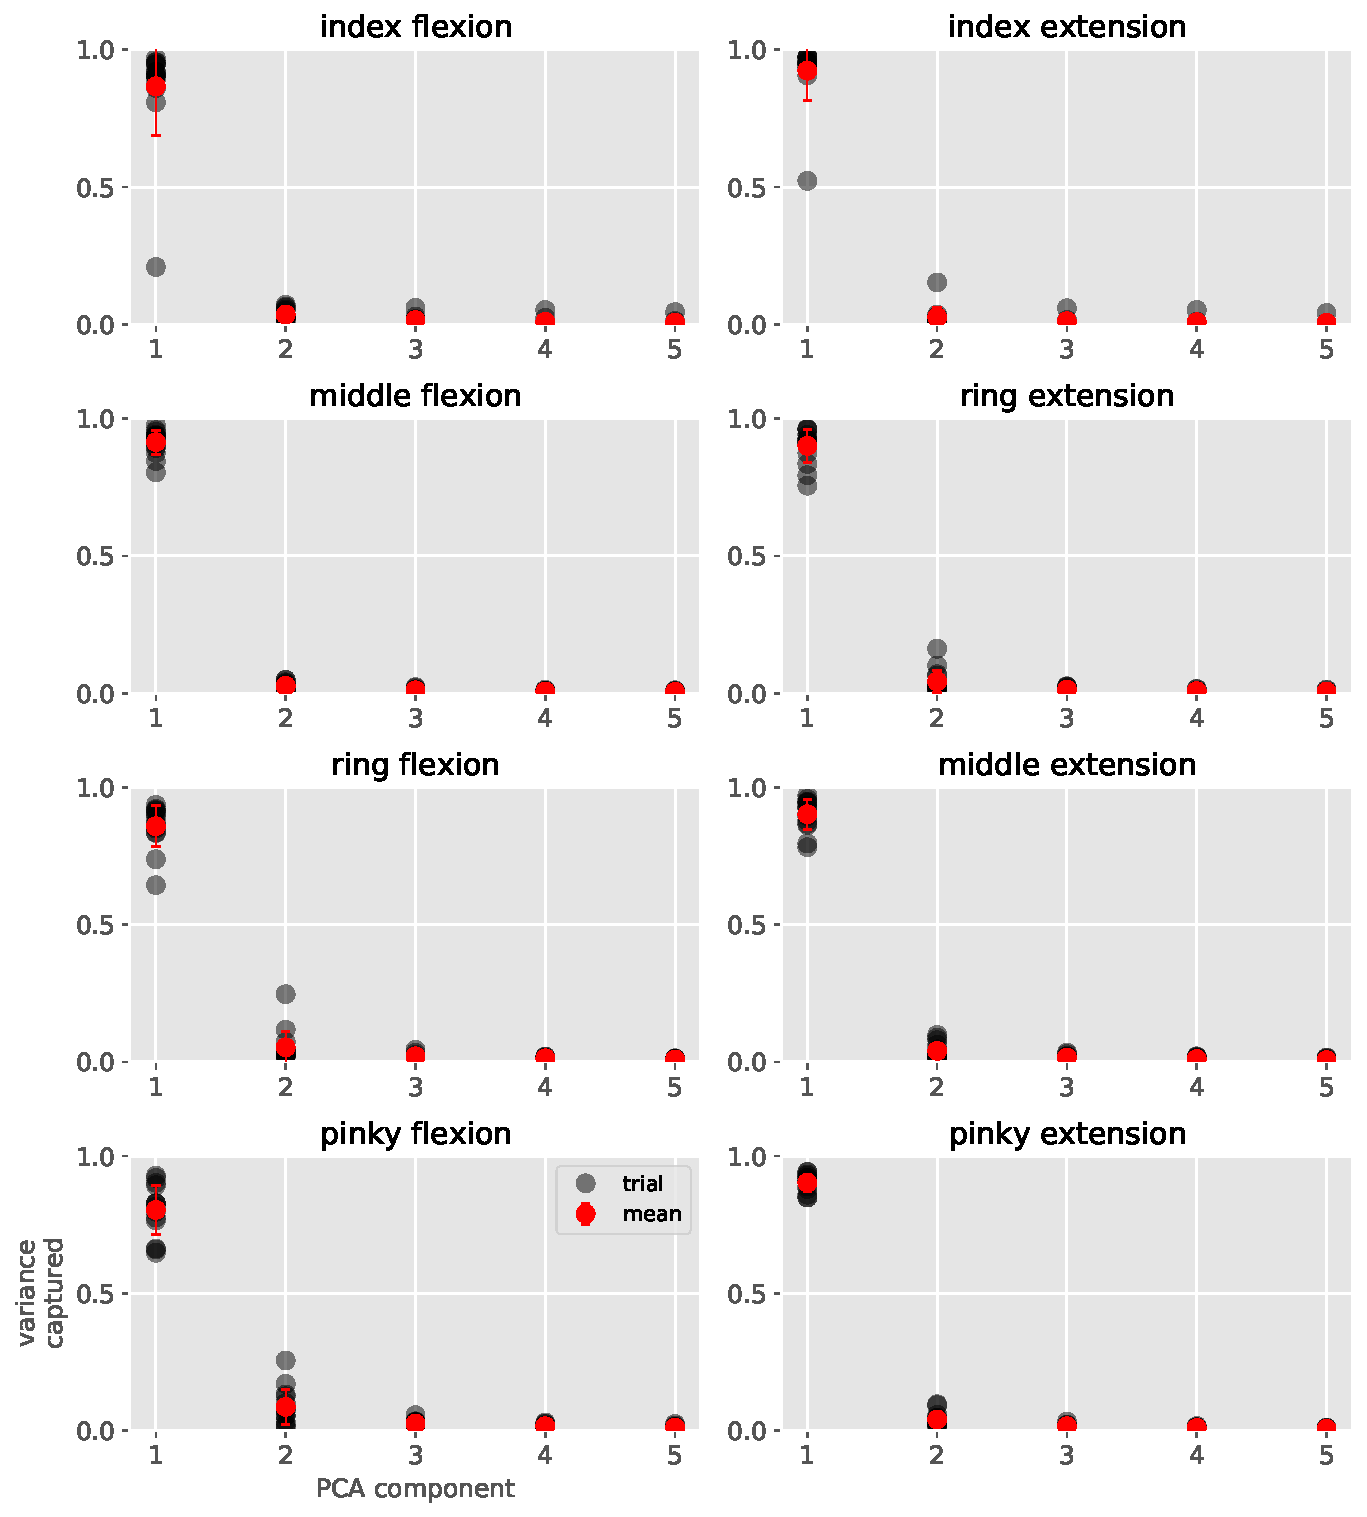
\includegraphics[width=0.2\textwidth]{images/data_analysis/fingers/PCA_variances.pdf}
% \caption{Fraction of variance captured by the top 5 principle components for trials of single finger extensions and flexions. PCs were computed for individual trials. Trials were recorded from one subject for 10s each trial with finger movement frequency approximately 1Hz. Three blocks each with one trial per finger movement were recorded per day for 5 days for a total of 15 trials per finger. Electrodes were not removed between blocks but were removed between days. Each trial displays a single high-variance PC component.}\label{fig:PCA_variances}
% \end{figure}

% We next asked, since each trial appeared to be dominated by a single principle component, whether this top component was stable across trials and across days. If the top component is stable, it implies that the recording apparatus is robust to electrode movement between sessions. The top components for each movement after running PCA on each trial are shown in \Cref{fig:PCA_components}. While it is not typical to run PCA on individual trials, for the purpose of visually inspecting the PCA weights over EMG channels it is used here.

% \begin{figure}[H]
% \phantomsection\label{fig:PCA_components}
% \centering
% 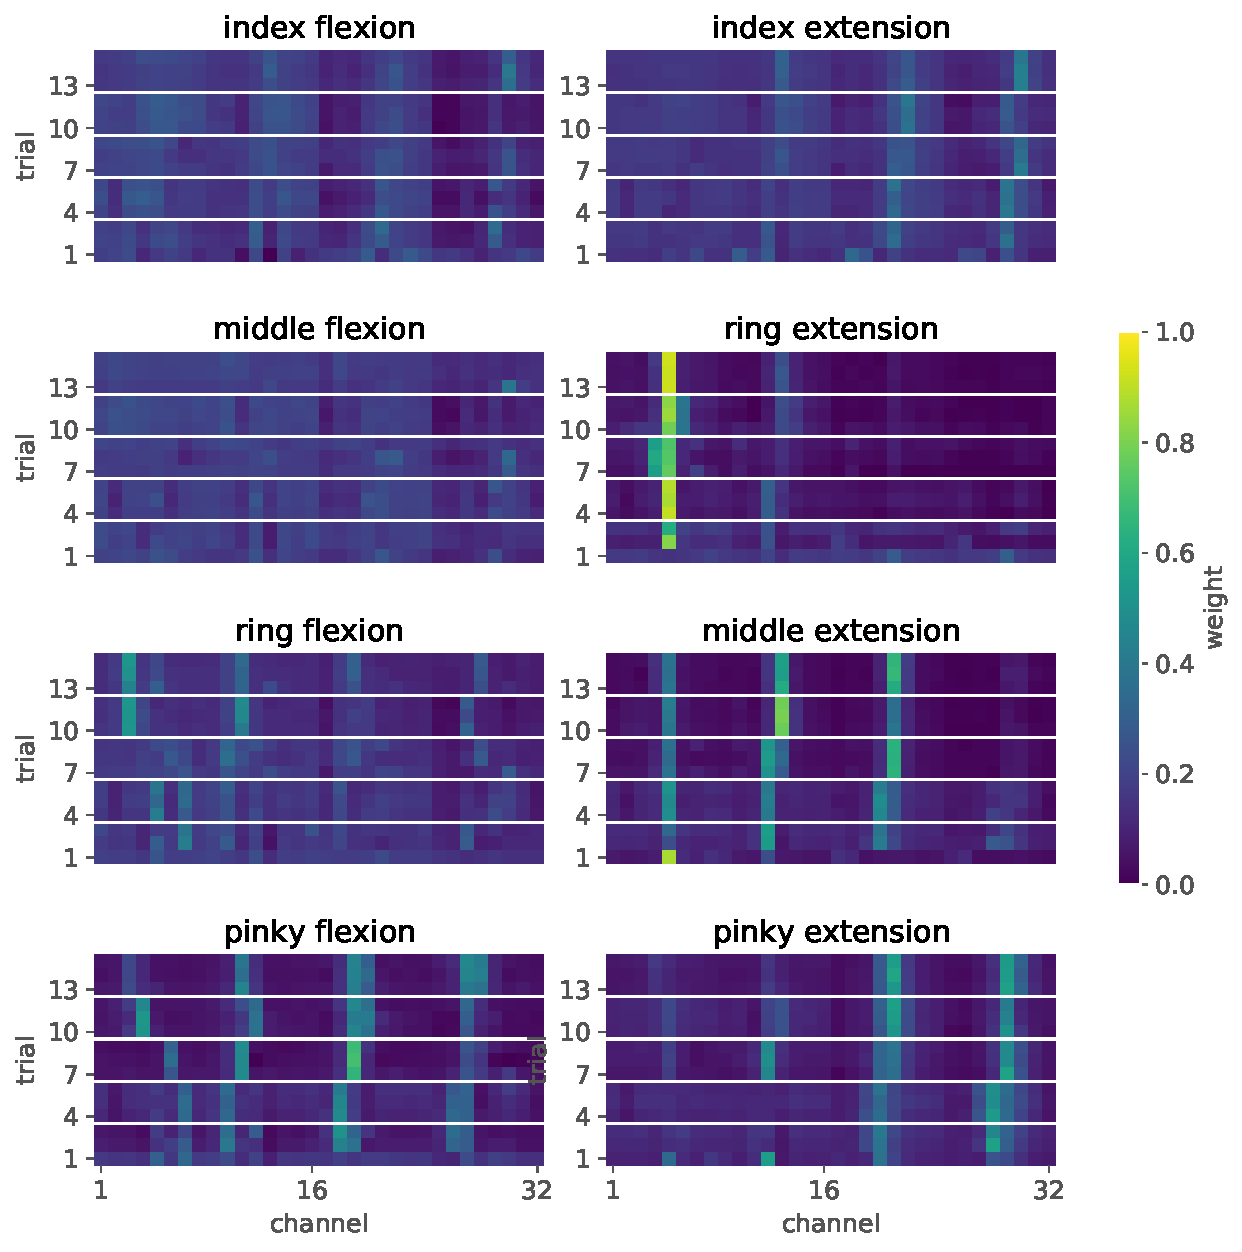
\includegraphics[width=0.2\textwidth]{images/data_analysis/fingers/PCA_components.pdf}
% \caption{The top principle component from each single finger movement trials plotted as weights across channels. PCA was computed for each trial individually. White horizontal lines show breaks between days when electrodes were removed and reapplied. Each trial's top component is relatively stable across trials and across days, though there is drift and dropout of weights. Measures to increase cross-session stability are discussed in the main text. Movements appear to vary between strong localization on single channels and broad activation across channels.}\label{fig:PCA_components}
% \end{figure}

% The results here suggest that, at least up to linear decompositions, the features of low-contraction movements is relatively robust across sessions. As discussed in {section:next\_steps}, we will construct more reliable means to place electrodes on subjects' forearms to further increase repeatability. Another aspect of these results is our assumption subjects are producing the same contraction each time they move their finger, and at the same contraction level. That is, we assume they are recruiting the same motor units each movement. This may not be the case, and constructing new analyses which infer motor unit activations may be useful to mitigate this issue.









\subsection{UMAP}

UMAP the data to motivate the nonlinear manifold, the “fingers” of the subspaces, and the “honing” idea – this supports the weird data manifold
Do a comparison on synthetic data to hammer the point home – compare to 64D Gaussian distribution with matching statistics..

\subsection{Toy GMM model demonstration X-pattern of trajectories}

Show how PCA fails to capture these statistics. Motivate the gaussian mixture model, even if these are overfit; we don't need these models to generalize, we're using them for summary statistics, like a filter.



\section{Subspace Confinement}

\begin{figure}[H]
  \centering
    \includegraphics[width=1.0\textwidth]{more_results/gmms/PCA_rank_fig.pdf}
    \caption[Explanatory Mixture Model]{The variables here are: the rank (number of rank-1 components making up the mixture), the ratio of the variance to the covariance of those components, and the "mixing" of each rank-1 component which effectively increases the rank of the mixture, if we assume to be a single Gaussian. We can see how as the variance begins to dominate the mixture looks more like a multivariate Gaussian. When components mix (without changing the overall variance to covariance ratio), we have a similar result due, however, to inability for PCA to model such a mixture as a single Gaussian. The 2D trajectory plots are shown for reference, but this effect is happening in the full 64D space, the values of the decoder are not a factor in this effect. See how PCA mischaracterizes the distribution in the mixed case, but fares well in the unmixed and high variance cases. This motivates our use of mixture models, which explicitly attempts to fit multiple Gaussians and can thus deal with mixing. Note that the effect here is slight, but demonstrates the principle of interest.}\label{fig:toy_model}
\end{figure}
  
How to transform gaussians into 2D
  
\begin{align}
    x &\propto N(\mu, \Sigma) \\ 
    y &= Ax + b \\ 
  y &\propto N(A\mu + b, A\Sigma A^T) \\ 
\end{align}

Do subjects who are less “confined” (constrained) are expected to perform better?



\section{Gaussian Mixtures}


\subsection{GMMs vs PCA}

\begin{figure}[H]
  \centering
    \includegraphics[height=0.8\textheight]{more_results/gmms/gmm_vs_pca.pdf}
    \caption[GMMs and PCA Covariance]{Compare the covariances of GMM fits to the covariances of individual PCA modes.}\label{fig:gmm_vs_pca}
\end{figure}


\subsection{Example GMMs}

% PRIOR %
\begin{figure}[H]
  \centering
  \begin{minipage}{0.49\textwidth}
    \includegraphics[width=\textwidth]{more_results/gmms/subject_10_movement_gmm.pdf}
    \subcaption{}
  \end{minipage}%
  \begin{minipage}{0.49\textwidth}
    \includegraphics[width=\textwidth]{more_results/gmms/subject_9_calibration_gmm.pdf}
    \subcaption{}
  \end{minipage}
  \caption[Example prior GMMs]{CAPTION}\label{fig:example_prior_gmms}
\end{figure}

% TRIAL %
\begin{figure}[H]
  \centering
    \includegraphics[height=0.8\textheight]{more_results/gmms/subject_1_trial_gmm.pdf}
    \caption[Subject 1 trial GMMs overlayed on trajectories]{CAPTION}\label{fig:example_1_trial_data_gmms}
\end{figure}

\begin{figure}[H]
  \centering
    \includegraphics[height=0.8\textheight]{more_results/gmms/subject_35_trial_gmm.pdf}
    \caption[Subject 35 trial GMMs overlayed on trajectories]{CAPTION}\label{fig:example_35_trial_data_gmms}
\end{figure}


\begin{figure}[H]
  \centering
  \begin{minipage}{0.49\textwidth}
    \includegraphics[width=\textwidth]{more_results/gmms/subject_1_gmms.pdf}
    \subcaption{}
  \end{minipage}%
  \begin{minipage}{0.49\textwidth}
    \includegraphics[width=\textwidth]{more_results/gmms/subject_14_gmms.pdf}
    \subcaption{}
  \end{minipage}
  \caption[Example GMMs for subjects 1 and 14]{CAPTION}\label{fig:example_gmms}
\end{figure}

\begin{figure}[H]
  \centering
  \begin{minipage}{0.49\textwidth}
    \includegraphics[width=\textwidth]{more_results/gmms/subject_37_trial_gmms.pdf}
    \subcaption{}
  \end{minipage}%
  \begin{minipage}{0.49\textwidth}
    \includegraphics[width=\textwidth]{more_results/gmms/subject_42_trial_gmms.pdf}
    \subcaption{}
  \end{minipage}
  \caption[Example trial GMMs for subjects 37 and 42]{CAPTION}\label{fig:example_trial_gmms}
\end{figure}


\subsection{GMM Pseudo-derivative}

\begin{figure}[H]
  \centering
    \includegraphics[width=\textwidth]{more_results/gmm_diffs/mean_gmm_differences.pdf}
    \caption[Mean GMM differences over subjects]{CAPTION}\label{fig:gmm_diffs}
\end{figure}

\begin{figure}[H]
  \centering
    \includegraphics[width=\textwidth]{more_results/gmms/gmm_wasserstein.pdf}
    \caption[Wasserstein distance between GMMs]{CAPTION}\label{fig:gmm_w2}
\end{figure}


\subsection{GMM Effective Rank}

\begin{figure}[H]
  \centering
    \includegraphics[width=\textwidth]{more_results/gmms/gmm_rank.pdf}
    \caption[Effective rank of GMMs]{CAPTION}\label{fig:gmm_rank}
\end{figure}

\begin{figure}[H]
  \centering
    \includegraphics[height=0.8\textheight]{more_results/gmms/rank_vs_reward.pdf}
    \caption[Effective rank]{CAPTION}\label{fig:rank_vs_reward}
\end{figure}


\subsection{GMM Entropy}

\begin{figure}[H]
  \centering
    \includegraphics[width=\textwidth]{more_results/gmms/entropy_gmms.pdf}
    \caption[Entropy of subject GMMs]{CAPTION}\label{fig:gmm_entropies}
\end{figure}

\begin{figure}[H]
  \centering
    \includegraphics[width=\textwidth]{more_results/gmms/entropy_diffs.pdf}
    \caption[Successive GMM entropy differences]{CAPTION}\label{fig:gmm_entropy_diffs}
\end{figure}


\subsection{Log Transforming the Data}

Show gaussian mixture fitting, show how they compare to data, show how stats of these change over trials

% PDF when transforming gaussian rv to log-gaussian rv https://stats.stackexchange.com/questions/214997/multivariate-log-normal-probabiltiy-density-function-pdf
% PDF when exponentiating gaussian to get lognormal? gauhttps://stats.stackexchange.com/questions/89970/exponential-of-a-standard-normal-random-variable


\subsection{Influence of Natural Repertoire}

Statistical distance between prior data and trial data
Mahalanobis distance, but this breaks down for multi-model data
Is there a metric we can use to measure similarity between these two datasets?
Subjects are hard-constrained by their hands physiology, but we think theyre also soft-constrained by their natural movement repertoire. We suggest casting this as a constrained policy optimization problem, where there is a regularization of the policy based on the prior movement data, which we suggest captures these natural constraints. The alternative we offer here is a norm-minimizing solution.
This is connected to the task-space vs. null-space activity as the norm-minimizing solution effectively ceases to move in the nullspace of the task
Fit GMMs to the trial and prior data, visualization these fits


Do we see a bias from natural statistics to trial statistics?
Do subjects avoid distribution mismatch between their base/prior/default policy and their optimal policy? How do they efficiently explore and use this new data to update their internal model?
What exploration strategy does a subject use to avoid mismatch? I.e. does variability in control/task space help or hurt subjects?




\cleardoublepage\printendnotes%
\ifSubfilesClassLoaded{%
    \newpage%
    \bibliography{../bib/bibliography}%
}{}%
\end{document}